\documentclass[11pt]{article}

\usepackage[a4paper,margin=0.85in]{geometry}
\usepackage{amsmath,amssymb}
\usepackage{booktabs}
\usepackage{graphicx}
\usepackage{hyperref}
\usepackage[T1]{fontenc}
\usepackage{lmodern}
\usepackage{microtype}
\hypersetup{hidelinks}

\graphicspath{{assets/generated/}}
\newcommand{\NoSkillMSE}{$5.932\times10^{-3}$}
\newcommand{\CheckpointTrainMSE}{$1.382\times10^{-4}$}
\newcommand{\CheckpointValMSE}{$1.803\times10^{-4}$}
\newcommand{\BaselineTrainMSE}{$3.236\times10^{-5}$}
\newcommand{\BaselineValMSE}{$3.504\times10^{-5}$}
\newcommand{\HigherRateValMSE}{$1.606\times10^{-2}$}
\newcommand{\TinyRateValMSE}{$1.923\times10^{-1}$}
\newcommand{\RawInputsValMSE}{$5.934\times10^{-3}$}
\newcommand{\SgdTrainMSE}{$3.747\times10^{-3}$}
\newcommand{\SgdValMSE}{$4.270\times10^{-3}$}
\newcommand{\SelectedName}{S4}
\newcommand{\SelectedValMSE}{$5.502\times10^{-8}$}
\newcommand{\SelectedEpoch}{4985}
\newcommand{\SelectedTrainMSE}{$4.554\times10^{-8}$}
\newcommand{\SelectedArchitecture}{3 hidden layers of 16 + 16 + 16}
\newcommand{\SelectedActivation}{tanh}
\newcommand{\SelectedRate}{$1\times10^{-3}$}
\newcommand{\SelectedParams}{641}
\newcommand{\BaselineParams}{49}
\newcommand{\SearchTrials}{6}
\newcommand{\ImprovementRatio}{637}
\newcommand{\MaxResponseError}{$6.652\times10^{-3}$}
\newcommand{\TestMSE}{$3.077\times10^{-5}$}
\newcommand{\TestRMSE}{0.0055470}
\newcommand{\TestRtwo}{0.9936}
\newcommand{\TailRMSE}{0.0195621}
\newcommand{\SelectedTestMSE}{$6.373\times10^{-8}$}
\newcommand{\SampleRows}{%
$P$ (N) & $1.000\times10^{4}$ & $9.995\times10^{3}$ & $7.000\times10^{2}$ & $7.069\times10^{2}$ \\
$E$ (Pa) & $3.000\times10^{10}$ & $3.000\times10^{10}$ & $3.000\times10^{9}$ & $3.023\times10^{9}$ \\
$L$ (m) & $3.000\times10^{0}$ & $3.014\times10^{0}$ & $1.155\times10^{0}$ & $1.157\times10^{0}$ \\
$I$ (m$^4$) & $1.100\times10^{-4}$ & $1.097\times10^{-4}$ & $5.196\times10^{-5}$ & $5.174\times10^{-5}$ \\
$y$ (m) & -- & $5.544\times10^{-2}$ & -- & $7.257\times10^{-2}$ \\
}
\newcommand{\SearchRows}{%
S1 & $[16]$ & tanh & $1\times10^{-3}$ & 1500 & $5.78\times10^{-5}$ & $7.28\times10^{-5}$ \\
S2 & $[16, 16]$ & tanh & $1\times10^{-3}$ & 1500 & $1.41\times10^{-6}$ & $3.44\times10^{-6}$ \\
S3 & $[16, 16, 16]$ & tanh & $1\times10^{-3}$ & 1500 & $1.47\times10^{-6}$ & $2.71\times10^{-6}$ \\
S4 & $[16, 16, 16]$ & tanh & $1\times10^{-3}$ & 5000 & $4.55\times10^{-8}$ & $5.50\times10^{-8}$ \\
S5 & $[16, 16]$ & tanh & $1\times10^{-3}$ & 5000 & $2.05\times10^{-7}$ & $4.28\times10^{-7}$ \\
S6 & $[32, 32]$ & relu & $1\times10^{-3}$ & 1500 & $1.55\times10^{-6}$ & $4.52\times10^{-6}$ \\
}

\newcommand{\answer}[2]{\par\noindent\textbf{#1.} #2\par}

\begin{document}
\begin{center}
  {\large Data-Driven Methods in Engineering\par}
  \vspace{0.4em}
  {\LARGE\bfseries Cantilever NN Surrogate: Instructor Baseline\par}
  \vspace{0.3em}
  {NTUA School of Civil Engineering\par}
\end{center}

\noindent This is one reproducible Python example, not a unique numerical answer. Run the script in \texttt{src/} with \texttt{uv} to regenerate the figures, numerical values, and \texttt{summary.json}. The seed is 20261104. The split contains 1800 training, 600 validation, and 600 test observations. The starting model has 1 hidden layer of 4 tanh neurons and learning rate $10^{-4}$. Its inputs are standardized using training-set statistics; the target stays in metres for the starting model and the Part~C probes. All runs use Adam and batch size 64 except the SGD probe. Part~B uses 500 epochs; the unchanged Part~C reference, all Part~C probes, and Part~D trials use 1500 epochs. Our Part~D search tries \SearchTrials\ configurations with at most \SearchMaxWidth\ neurons per layer; this cap is ours, students may try anything. The script records full training- and validation-set MSE after each epoch.

\section*{A. Dataset and mechanical expectations}
The nominal prediction from the beam equation is
\[
  \delta_0=\frac{10\,000(3)^3}{3(30\times10^9)(8\times10^{-5})}=0.0375\ \mathrm m.
\]
The sampled moments (population-style standard deviations) are:
\begin{center}
\begin{tabular}{@{}lrr@{}}
\toprule
Quantity & Sample mean & Sample standard deviation \\
\midrule
\SampleRows
\bottomrule
\end{tabular}
\end{center}

\begin{figure}[htbp]
  \centering
  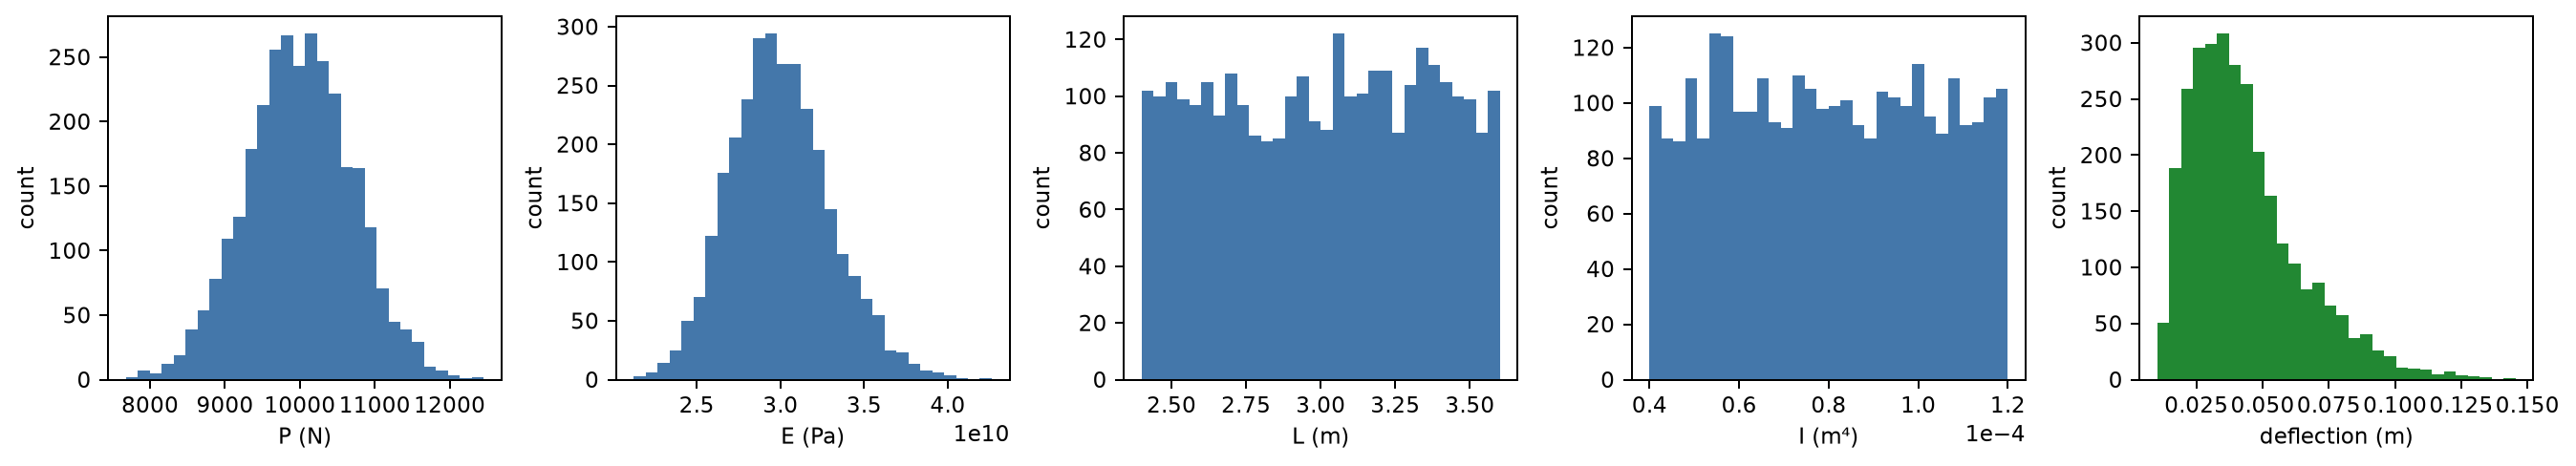
\includegraphics[width=\textwidth]{input_histograms.png}
  \caption{The sampled inputs and analytical deflection. Counts use 30 bins per histogram.}
\end{figure}

\answer{A1}{The moments are close to their targets, not identical: 3000 independent samples still have sampling variation. The lognormal conversion is essential for $E$: setting the underlying normal mean to $30\times10^9$ would be incorrect.}
\answer{A2}{The sampled deflection is right-skewed and predominantly positive. Negative values are possible because $P$ is normally distributed. Deflection combines 4 independent inputs, with $P$ and $L^3$ in the numerator and $E$ and $I$ in the denominator; no single input distribution determines its histogram.}
\answer{A3}{For small relative perturbations, $d\delta/\delta\approx dP/P-dE/E+3dL/L-dI/I$. The approximate standard-deviation contributions are 7\% ($P$), 10\% ($E$), 35\% ($L$), and 29\% ($I$). Thus $L$ and $I$ should dominate, followed by $E$ and $P$. The wider ranges make this first-order comparison less accurate; it is not an exact variance decomposition.}

\section*{B. Starting model}
\answer{B1}{The training inputs and targets have shapes $1800\times4$ and $1800\times1$. Validation and test each use $600\times4$ inputs and $600\times1$ targets. A batch of $b$ rows produces $b\times1$ predictions.}
\answer{B2}{A composition of affine layers remains affine. The nonlinear tanh activation lets the network approximate the reciprocal and cubic dependence in the beam equation over the prescribed ranges.}
\answer{B3}{Training MSE is the average squared difference between analytical reference deflections and training predictions, in m$^2$. A decrease means better fit to those observations; it alone says nothing about generalization. The starting model ends with train MSE \BaselineTrainMSE\ m$^2$ and validation MSE \BaselineValMSE\ m$^2$; its history appears in Figure~\ref{fig:baseline-loss}.}
\answer{B4}{Adam maintains running averages of gradients and squared gradients. The first gives a momentum-like direction; the second adapts the size of each parameter update.}
\answer{B5}{With 1800 training observations and batch size 64, 1 epoch has $\lceil1800/64\rceil=29$ batches; the last contains 8 observations.}
\answer{B6}{At epoch 500, both curves are still decreasing. This suggests that more training could improve the fit, but the plot alone cannot show how much or whether validation MSE will eventually turn upward. Part~C tests this by training the unchanged model for 1500 epochs.}

\begin{figure}[htbp]
  \centering
  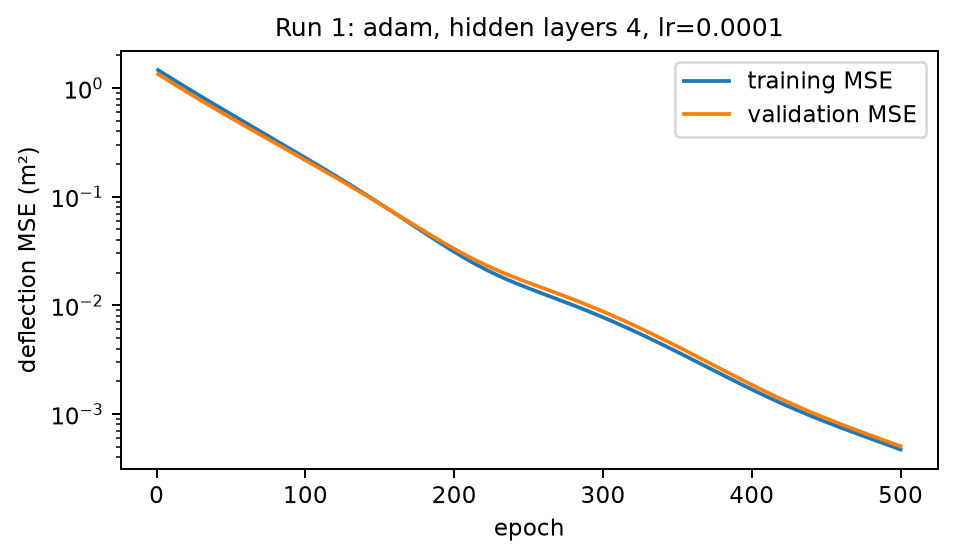
\includegraphics[width=0.68\textwidth]{loss_run_1.png}
  \caption{The 4-neuron starting model after 500 epochs; MSE uses a logarithmic y-axis.}\label{fig:baseline-loss}
\end{figure}

\section*{C. Controlled training probes}
\noindent At 1500 epochs, the unchanged 4-neuron model reaches training MSE \ReferenceTrainMSE\ m$^2$ and validation MSE \ReferenceValMSE\ m$^2$, compared with \BaselineTrainMSE\ and \BaselineValMSE\ m$^2$ at 500 epochs. Longer training alone helps a lot, but it is not enough: the reference is still \ImprovementRatio\ times above the Part~D winner's validation MSE, so students must also change the model or training setup.
\subsection*{Learning rate}
\answer{C1}{With the same architecture and standardized inputs, $10^{-5}$ gives validation MSE \TinyRateValMSE\ m$^2$ after 1500 epochs: its updates are too small to make enough progress. The reference rate $10^{-4}$ gives \ReferenceValMSE\ m$^2$. At $10^{-1}$, validation MSE is \HigherRateValMSE\ m$^2$; its loss spikes show updates too large for stable convergence here.}

\begin{figure}[htbp]
  \centering
  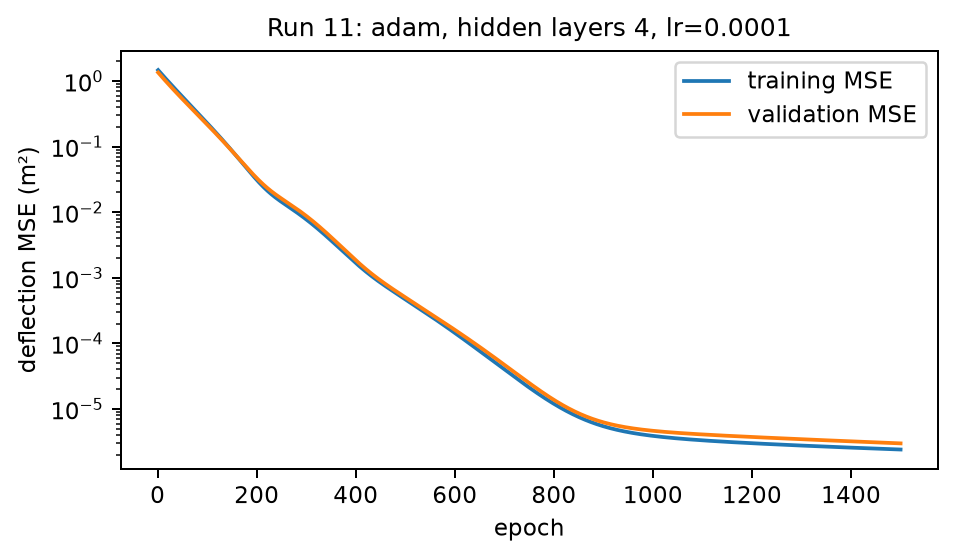
\includegraphics[width=0.48\textwidth]{loss_run_11.png}\hfill
  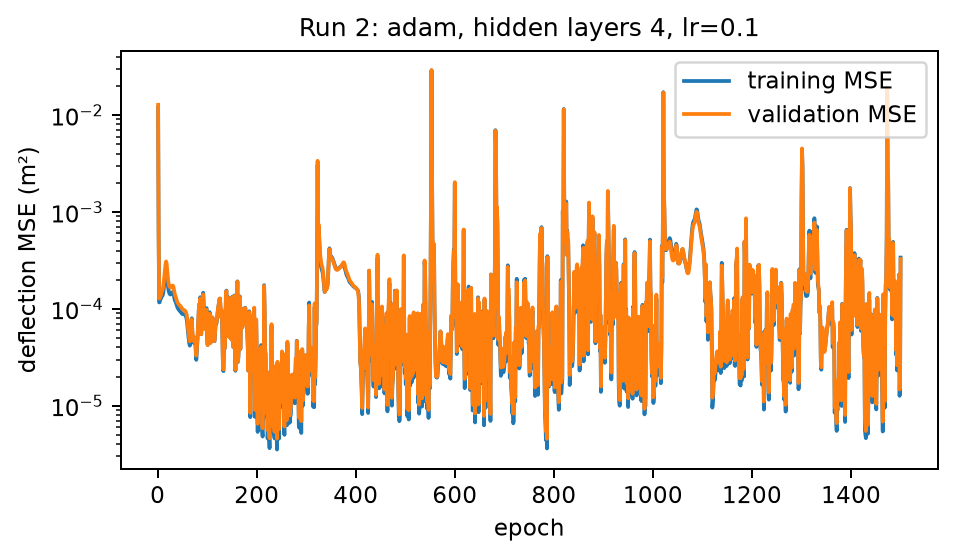
\includegraphics[width=0.48\textwidth]{loss_run_2.png}
  \caption{Training and validation MSE over 1500 epochs on a logarithmic y-axis: unchanged rate $10^{-4}$ (left) and unstable $10^{-1}$ (right).}\label{fig:losses}
\end{figure}

\begin{figure}[htbp]
  \centering
  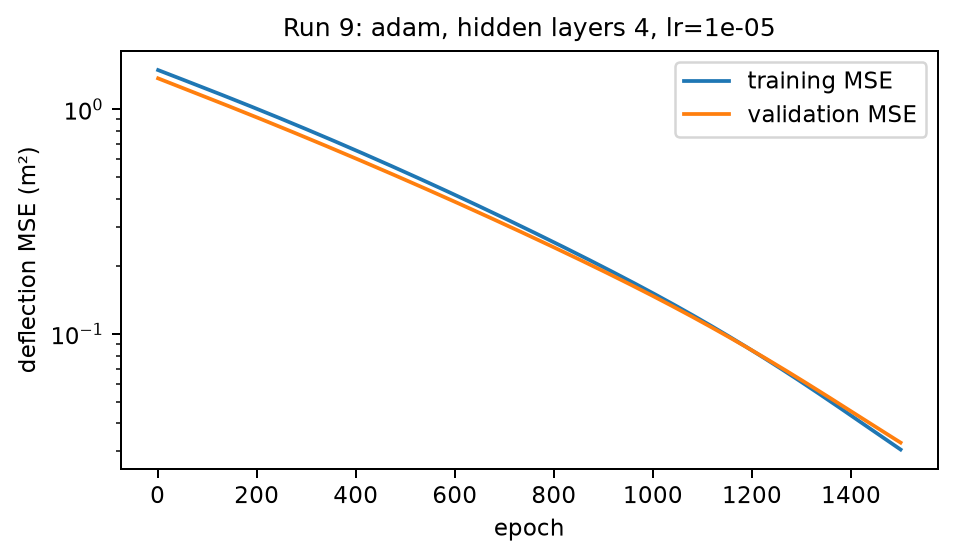
\includegraphics[width=0.68\textwidth]{loss_run_9.png}
  \caption{At $10^{-5}$, the starting architecture makes little progress within the epoch budget; MSE uses a logarithmic y-axis.}
\end{figure}

\subsection*{Input standardization}
\answer{C2}{Using raw SI inputs at the starting learning rate gives validation MSE \RawInputsValMSE\ m$^2$. The input magnitudes span roughly $10^{-4}$ to $10^{10}$, so a shared optimizer step has to work with very different weight-gradient scales. The result illustrates why input standardization matters here; numerical failure would also be a valid observation.}

\subsection*{Optimizer}
\answer{C3}{Plain SGD with the 1500-epoch reference settings gives training MSE \SgdTrainMSE\ m$^2$ and validation MSE \SgdValMSE\ m$^2$, compared with \ReferenceValMSE\ m$^2$ for Adam. Its loss decreases much more slowly. With the target measured in metres, gradients can be small; the same fixed learning rate need not give SGD the useful per-parameter step sizes provided by Adam's running averages. This comparison is specific to these settings, not a general ranking of optimizers.}
\answer{C4}{No run shows the sustained decrease in training MSE alongside a rise in validation MSE that would indicate overfitting. The poorer runs instead show slow progress or large fluctuations, often in both curves. A small train--validation gap alone does not mean the model has learned enough.}

\begin{figure}[htbp]
  \centering
  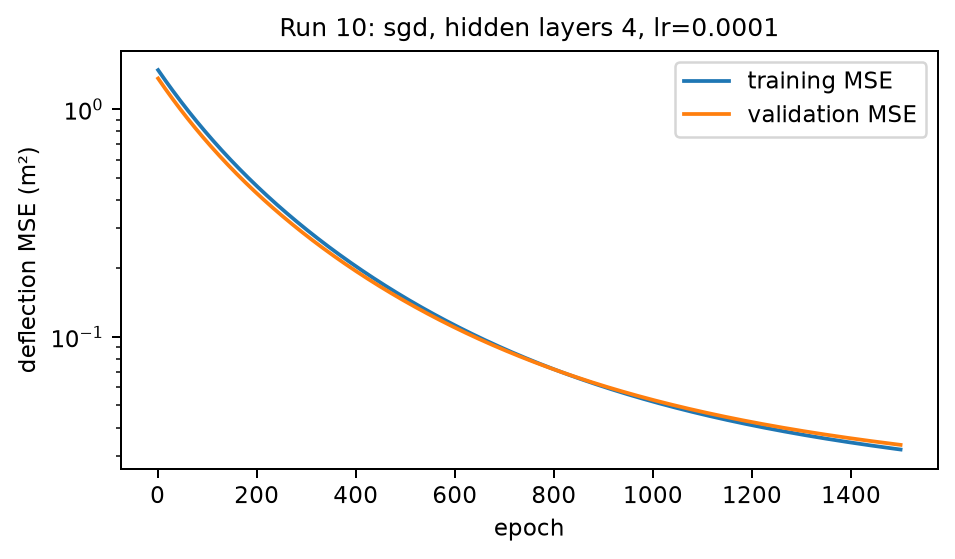
\includegraphics[width=0.68\textwidth]{loss_run_10.png}
  \caption{Training and validation MSE for plain SGD with the 4-neuron architecture and rate $10^{-4}$ over 1500 epochs.}
\end{figure}

\section*{D. Open model improvement}
\answer{D1}{The winning run has \SelectedArchitecture\ \SelectedActivation\ neurons and a linear output. It standardizes inputs using training-set statistics, has its target \SelectedTargetScaling\ (predictions are mapped back to metres), and uses Adam at learning rate \SelectedRate\ with batch size 64 and an epoch budget of 1500. It is the best of \SearchTrials\ searched configurations on one seed; the next-best configurations are within a factor of 2 to 3 of it, so this is not a unique or general optimum.}
\answer{D2}{Its final training MSE is \SelectedTrainMSE\ m$^2$ and validation MSE is \SelectedValMSE\ m$^2$, about \ImprovementRatio\ times lower than the 1500-epoch 4-neuron reference validation MSE \ReferenceValMSE\ m$^2$. Its loss history falls smoothly in plateau-and-drop steps with no spikes, and both curves are still slowly decreasing at epoch 1500, with validation about 2 times above training.}
\answer{D3}{The starting model has $(4\cdot4+4)+(4+1)=25$ trainable weights and biases. The winning model has \SelectedParams. More parameters help, but the count alone does not explain the result: the best searched 4-neuron model (more rate-tuned, same width as Part~B) reaches only \BestFourNeuronValMSE\ m$^2$, and deeper 8-neuron models with several times more parameters do not beat the winner.}
\answer{D4}{Compared with the 1500-epoch reference, the selected run uses width 8 instead of 4, a $30\times$ larger learning rate, and a standardized target. The search table supports three effects: the best configuration with the target left in metres reaches \BestRawTargetValMSE\ m$^2$ (target scaling helps about 3 times), the best ReLU configuration reaches \BestReluValMSE\ m$^2$ (tanh suits this smooth response), and the best 4-neuron configuration reaches \BestFourNeuronValMSE\ m$^2$ (width helps about 10 times). Extra depth did not help beyond this. These are single-seed comparisons across the grid, not controlled one-factor experiments.}

\begin{figure}[htbp]
  \centering
  \includegraphics[width=0.72\textwidth]{loss_run_\SelectedRun.png}
  \caption{Training and validation MSE for the selected model (\SelectedArchitecture, \SelectedActivation, learning rate \SelectedRate) over 1500 epochs.}\label{fig:selected-loss}
\end{figure}

\section*{E. Held-out and engineering evaluation}
\noindent The selected model has test MSE \TestMSE\ m$^2$, RMSE $\TestRMSE\ \mathrm m$, and $R^2=\TestRtwo$. For the highest 5\% of analytical test deflections, RMSE is $\TailRMSE\ \mathrm m$ (30 observations), about 4 times the overall RMSE.

\begin{figure}[htbp]
  \centering
  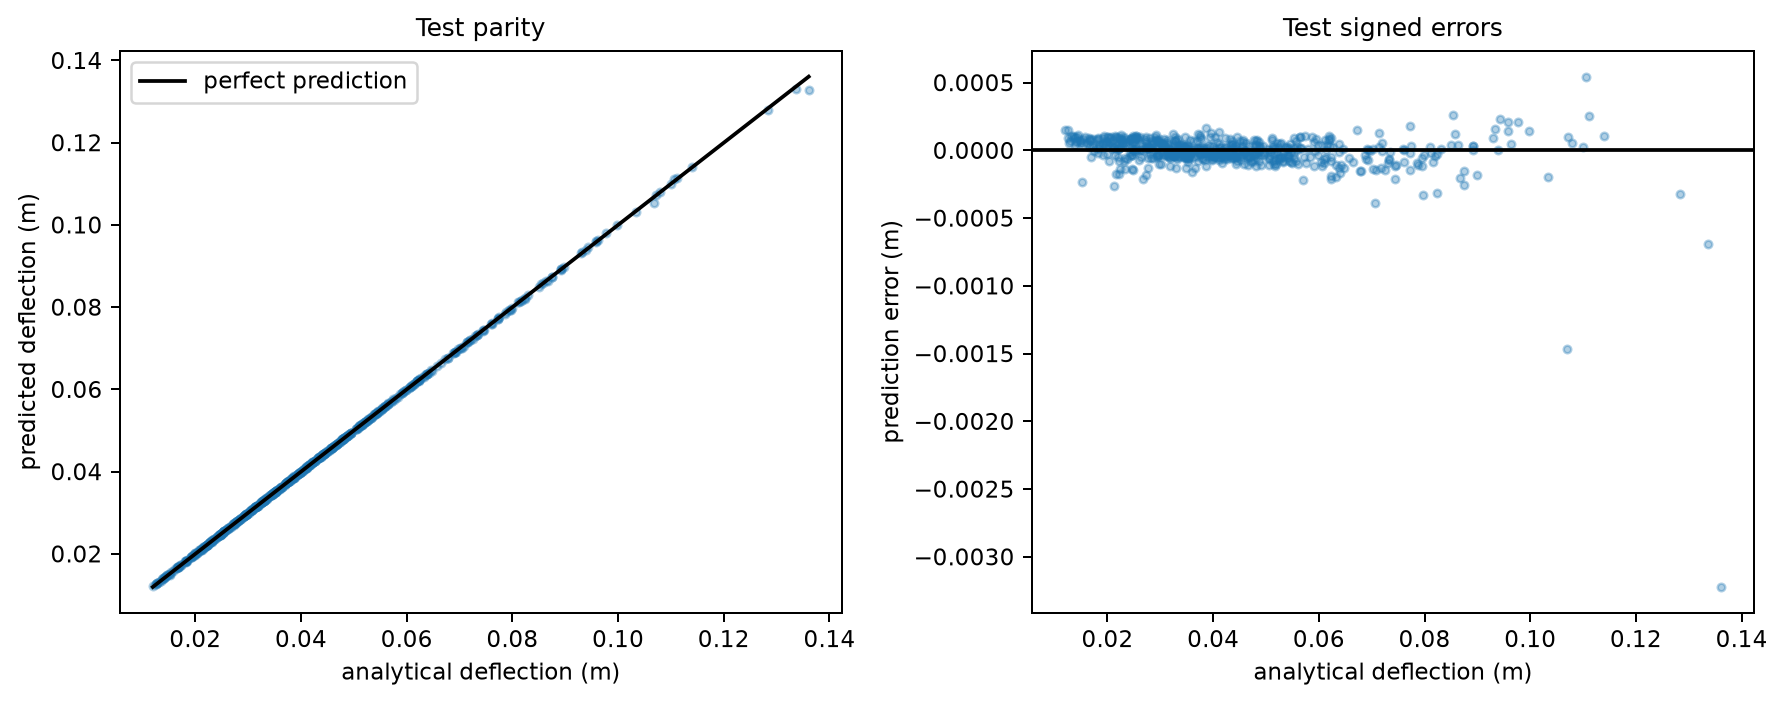
\includegraphics[width=0.9\textwidth]{test_diagnostics.png}
  \caption{Held-out test parity and signed error against analytical deflection. The diagonal and zero line mark perfect prediction.}
\end{figure}

\answer{E1}{The test fit is very close: almost all errors lie within about $\pm3\times10^{-4}$ m. The signed-error plot shows what $R^2$ hides: the largest errors are underestimates at the highest deflections, about $-3.2\times10^{-3}$ m at $0.136$ m and $-1.5\times10^{-3}$ m near $0.107$ m. Errors at small deflections are tiny and slightly positive.}

\begin{figure}[htbp]
  \centering
  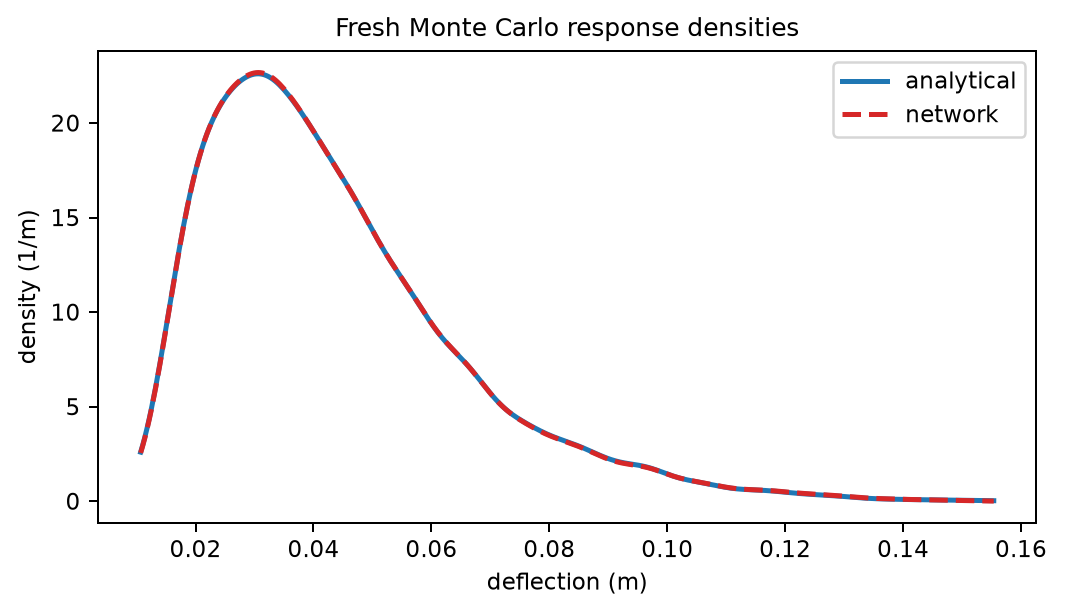
\includegraphics[width=0.68\textwidth]{mc_distribution.png}
  \caption{KDE curves for analytical and surrogate deflections on the same 10\,000 fresh Monte Carlo inputs. A shared bandwidth is used for comparison.}
\end{figure}

\begin{center}
\begin{tabular}{@{}lrrr@{}}
\toprule
Output & Mean (m) & Standard deviation (m) & 95th percentile (m) \\
\midrule
Analytical & \AnalyticalMean & \AnalyticalStd & \AnalyticalPnn \\
Surrogate & \SurrogateMean & \SurrogateStd & \SurrogatePnn \\
\bottomrule
\end{tabular}
\end{center}

\answer{E2}{The means, standard deviations, and 95th percentiles agree closely on paired Monte Carlo inputs. For example, the 95th percentiles are \AnalyticalPnn\ m and \SurrogatePnn\ m. The common inputs prevent sampling noise from obscuring model error.}
\answer{E3}{The upper-tail RMSE is about 4 times the overall RMSE, and the surrogate's 95th percentile is slightly below the analytical one. Large deflections are sparsely sampled and the largest ones are underestimated, so accuracy drops in the tail even though the fitted distribution looks accurate.}

\clearpage
\begin{figure}[htbp]
  \centering
  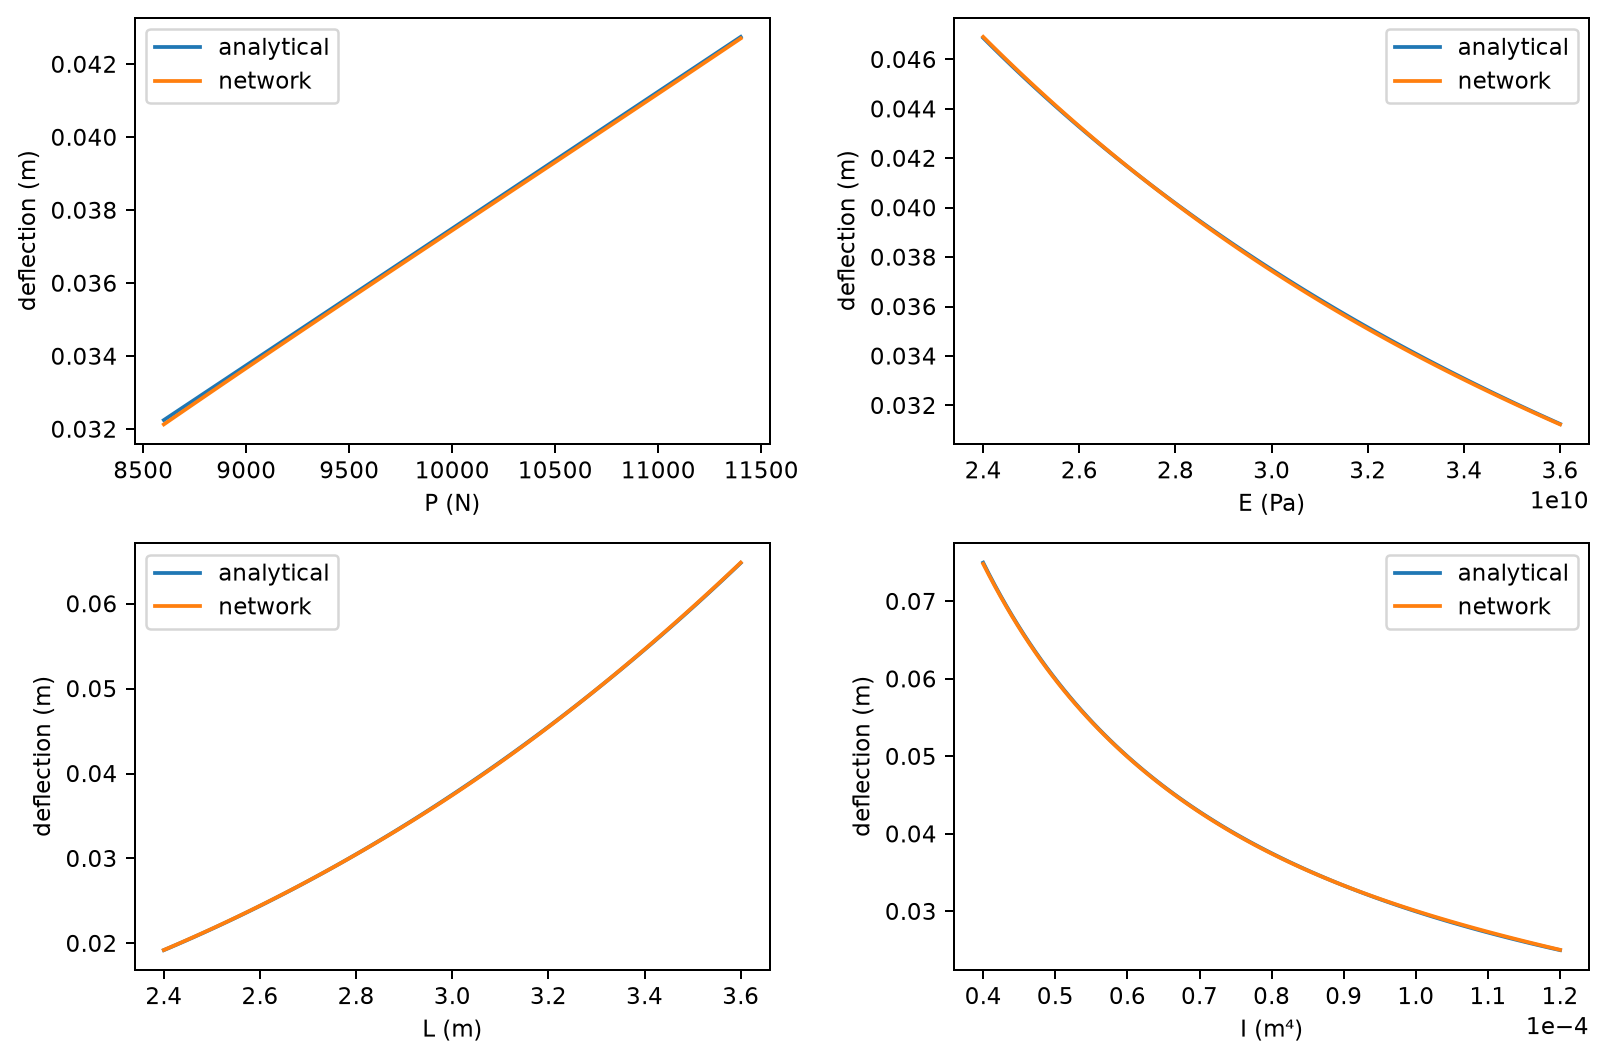
\includegraphics[width=0.85\textwidth]{response_curves.png}
  \caption{Single-input response curves, with other inputs held at nominal means.}
\end{figure}

\answer{E4}{The network tracks all 4 nominal response curves closely; the curves are nearly indistinguishable. The largest maximum absolute discrepancy among the 4 sweeps is on the $I$ sweep, approximately \MaxResponseError\ m.}
\answer{E5}{The analytical response is linear in $P$ and reciprocal in $E$. The network reproduces the near-straight $P$ curve and the curvature of $E$ across the selected ranges, with small deviations visible on close inspection.}
\answer{E6}{The curves are compatible with the A3 sensitivity prediction, but their vertical changes depend on the chosen sweep widths. Total variance also depends on the probability distributions and simultaneous variation of all 4 inputs; single-input curves do not allocate that variance.}

\end{document}
